%%「論文」,「レター」,「レター(C分冊)」,「技術研究報告」などのテンプレート
%% v3.3 [2020/06/02]
%% 1. 「論文」
\documentclass[technicalreport]{ieicej}
%\documentclass[invited]{ieicej}% 招待論文
%\documentclass[survey]{ieicej}% サーベイ論文
%\documentclass[comment]{ieicej}% 解説論文
%\usepackage[dvips]{graphicx}
%\usepackage[dvipdfmx]{graphicx,xcolor}
\usepackage[fleqn]{amsmath}
\usepackage{newtxtext}% 英数字フォントの設定を変更しないでください
\usepackage[varg]{newtxmath}% % 英数字フォントの設定を変更しないでください
\usepackage{latexsym}
%\usepackage{amssymb}
\usepackage[dvipdfmx]{graphicx}
\bibliographystyle{sieicej}
\graphicspath{ {./img/} }

\setcounter{page}{1}

\field{}
\jtitle{Beyond 5G高周波通信の空間分解能を 向上するための誘電体導波路の研究}
\etitle{Research on Dielectric Waveguides for Enhancing Spatial Resolution in Beyond 5G High Frequency Communications}
\authorlist{%
 \authorentry[mitani-reishi116@g.ecc.u-tokyo.ac.jp]{三谷怜司}{Reishi Mitani}{東京大学 〒113-0033 東京都文京区本郷 7-3-1}\MembershipNumber{}
 \authorentry[nakao@nakao-lab.org]{中尾彰宏}{Akihiro Nakao}{東京大学 〒113-0033 東京都文京区本郷 7-3-1}\MembershipNumber{}
 %\authorentry{和文著者名}{英文著者名}{所属ラベル}\MembershipNumber{}
 %\authorentry[メールアドレス]{和文著者名}{英文著者名}{所属ラベル}\MembershipNumber{}
 %\authorentry{和文著者名}{英文著者名}{所属ラベル}[現在の所属ラベル]\MembershipNumber{}
}
\affiliate[]{東京大学 〒113-0033 東京都文京区本郷 7-3-1}{The University of Tokyo, Graduate School of Interdisciplinary Information Studies 7-3-1, Hongo, Bunkyo-ku, Tokyo, 113-0033 Japan}
%\affiliate[所属ラベル]{和文所属}{英文所属}
%\paffiliate[]{}
%\paffiliate[現在の所属ラベル]{和文所属}
\jalcdoi{???????????}% ← このままにしておいてください

\begin{document}
\begin{abstract}
  5G・Beyond5Gで普及が期待されている高周波数の通信では
  帯域を広く利用することで大容量の通信が可能となる一方
  電波伝播の直進性や急激な減衰から利活用の困難さが指摘されている。
  我々は、ミリ波などの高周波数を利用する通信において、直進性や減衰性を逆に利用し、
  高空間分解能の通信に利活用することを考えている。
  一般に、ミリ波ではアレイアンテナを利用するビームフォーミングにより電波伝播の範囲を
  限定することが可能であるが、コストが高いなどの課題がある。
  本研究では、低コストでビームを絞るための誘電体導波路を用いたミリ波アンテナを設計・
  製作することを提案し
  シミュレーション評価によりその有用性を示す。
\end{abstract}
\begin{keyword}
%和文キーワード 4〜5語
Beyond5G
\end{keyword}
\begin{eabstract}
%英文アブストラクト 100 words
High-frequency communications,
which are expected to be widely used in 5G and Beyond5G,
enable high-capacity communications by using a wide bandwidth.
However, the linearity of radio wave propagation and rapid attenuation
have made it difficult to utilize high-frequency communications.
In this paper, we consider the use of millimeter waves and
other high-frequency communications for high-spatial-resolution communications
by taking advantage of their linearity and attenuation.
Generally, it is possible to limit the range of radio propagation by
beamforming using array antennas in millimeter-wave communications,
but there is a problem of high cost.
In this study,
we propose to design and fabricate a millimeter-wave antenna using
dielectric waveguides to narrow the beam at low cost,
and demonstrate its usefulness through simulation evaluation.
\end{eabstract}
\begin{ekeyword}
%英文キーワード
Beyond5G
\end{ekeyword}
\maketitle

\section{はじめに}

第5世代移動通信システム(5G)の商用サービスが2020年3月に開始され、
移動通信システムとしては初めて、28GHz帯を利用した広帯域高速通信が実用化された。
28GHz以上のミリ波の帯域の利用は今後拡大されることが予想される。

5G・Beyond5Gで普及が期待されている高周波数の通信では、
帯域を広く利用することで大容量の通信が可能となる一方、
電波伝播の直進性や急激な減衰から利活用の困難さが指摘されている。
また、ミリ波は高分解能があるにもかかわらず、
それを生かしたセキュリティを確立する方法が難しい。
ここでいうセキュリティというのは以下のことを示す。

\begin{itemize}
  \item デバイスが多い環境においては、それぞれのデバイスへの電波の割り当てが困難となる
  \item 渡すべきでない情報を他のデバイスに渡してしまうことがありえる
\end{itemize}

セキュリティを向上する既存の方法では以下の障害が存在する。
一つ目はミリ波専用の機器はハード、ソフトともに開発コストがかかるうえ、
ミリ波は波長が短く、より精密なエンジニアリングが必要となることである。
MIMOなどを実装し、ビームフォーミングを可能にすることでセキュリティ
を向上することも可能だが、これも開発と実装、そしてチューニングのコストがかかる。
二つ目はリードタイムが長いことで、ホーンアンテナなどの機器は納品までに時間がかかる。
これもより精密なエンジニアリングが必要となることに起因する。
3つ目にインフラが柔軟でないことがあげられる。
ホーンアンテナなどの機器は一度配置してしまうと場所を変えにくいため、
設計などに気を付けなければならない。

本論文の関連研究としてはまず、
NTT Docomoによる曲がるアンテナ
\cite{bending_antenna} \cite{leaky_wave_antenna_bent_dielectric}
があげられる。
誘電体導波路を曲げて漏れ出した電波を利用し、
エリアの拡張ができることを実証した。
送受信の可逆性により、曲げた箇所は送受信がともに可能なアンテナとなる上、
曲げる箇所を柔軟に変えることで電波の出るエリアを移動することが可能です。
また、シミュレーションで曲げた箇所からの電波の漏れ出しを可視化しており、
こちらの結果から入力電力の最大50\%程度が曲げた箇所から放出されることが
わかる。
他には誘電体導波路をより誘電率の高い物質ではさんだ場合、
はさんだ箇所から電波が漏れ出す現象を生かしたエリア構築の例がある。
この現象を利用すれば誘電体導波路を曲げずともエリア構築が可能となる上、
洗濯ばさみのような物質でエリア構築ができる手軽さがある。

本研究では、シミュレーションを用いて
誘電体導波路の最適な形状を割り出し、
それをもとに誘電体導波路アンテナの製作を行う。
製作したアンテナの反射率と指向性を測定し、
セキュリティへの有用性を確認する。

本論文の構成は次の通りである.次章では,本研究
に関連する技術について述べる.第3章,第4章では,
システム概要を示した提案手法と実際の実装について
まとめる.第5章にて,各ケースにおけるスループット
やFPSの評価を行い,第6章で今後の展望について考察
する.最終章にて本論文をまとめる.

\section{関連技術}

\subsection{既存の伝送媒体}

ミリ波の伝送媒体には主に以下が利用される。
\begin{itemize}
  \item 導波管
  \item 同軸ケーブル
  \item 誘電体導波路
\end{itemize}

導波管は誘電体または空気の周囲を導体で囲んだ断面形状をもち、衛星地球局で利用される。
ただ容易に曲げることができず、重いという制約がある。
同軸ケーブルは中心導体と外部導体が同心円状に配置された断面形状をもち、
おもにマイクロ波以下の周波数帯で利用される。
こちらは高周波数帯での損失が導波管よりも高いという制約がある。

誘電体導波路(\ref{fig:dielectric_waveguide})は棒状の誘電体の周囲を異なる誘電率を有する誘電体で囲んだ構造を持ち、
高周波数帯電波の伝送のために使われることが多い
導波管と同軸ケーブルを足して2で割ったような特徴を持ち、
損失は発生するが、同軸ケーブルよりは低い上、軽くて柔軟に曲げることができる。


\begin{figure}[tb]
  %\capwidth=60mm
  %\ecapwidth=60mm
  \begin{center}
    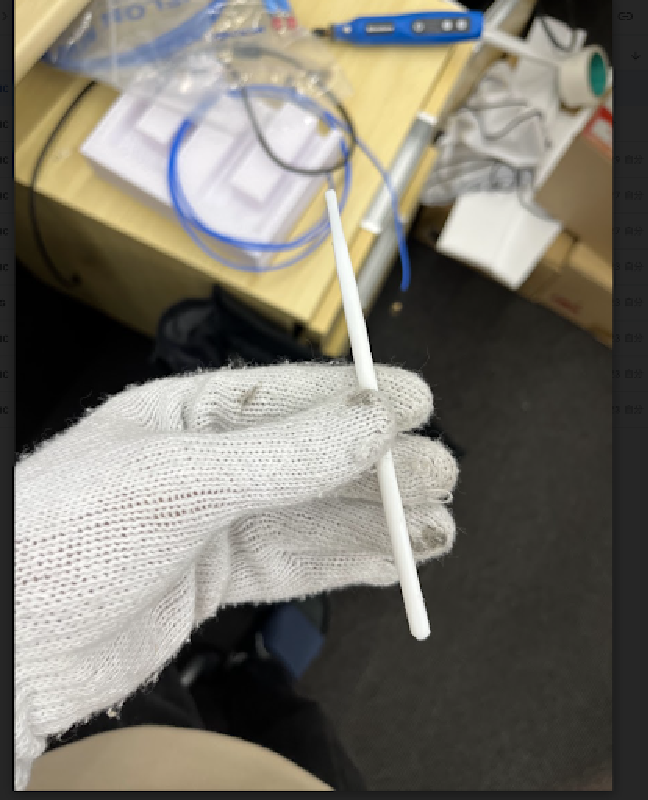
\includegraphics[bb=0 0 311 384, width=0.5\linewidth]{img/waveguide.pdf}
    \caption{誘電体導波路}
    \label{fig:dielectric_waveguide}
  \end{center}
\end{figure}

\subsection{誘電体導波路の先端から出る高分解能ビーム}

本研究では、予備実験にて誘電体導波路の先端から
高分解能ビームが出ていることを確認している。
予備実験では動画の送受信システムを60 GHz帯で構築し、
60GHzの電波の送信機を銅板で囲って電波を遮断した上で
導波路をアンテナ代わりに使う調査実験を行った。

実際に導波路を動かしたり、力を加えることで特徴を探したところ、
導波路の先端から高指向性のビーム状の電波が放出されることがわかった。
図\ref{fig:qualitative_experiment}
のように60GHzの動画送受信システムにおいて、
受信機に向けているときには動画は再生され、
ちょっとでも下に向けているときには動画が再生されない
現象を見つけることができた。

\begin{figure*}[t]
  %\capwidth=60mm
  %\ecapwidth=60mm
  \begin{center}
    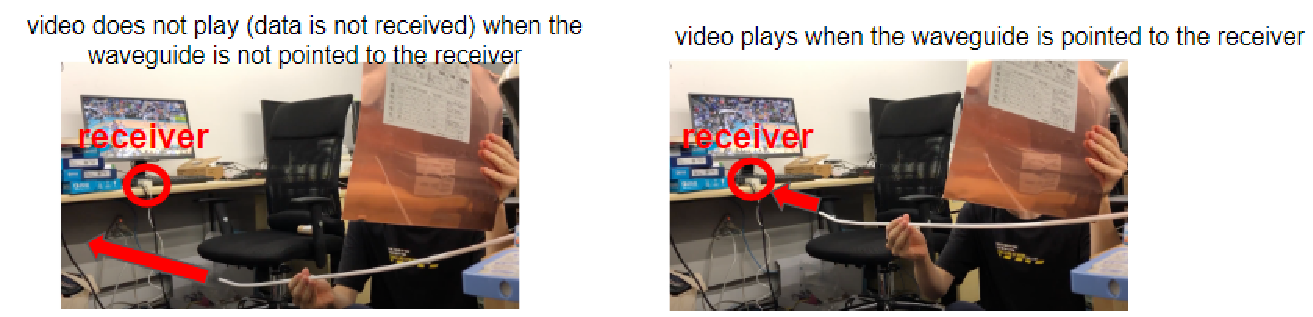
\includegraphics[bb=0 0 630.087950 152.271255, width=1.0\linewidth]{img/qualitative_experiment.pdf}
    \caption{誘電体導波路の予備実験}
    \label{fig:qualitative_experiment}
  \end{center}
\end{figure*}


\section{提案手法}

本研究では電波伝播の直進性や急激な減衰を利活用した
誘電体導波路を用いたミリ波アンテナを設計し製作する。
そしてシミュレーション評価だけでなく実際に作製したアンテナを用いた実験により、
セキュリティに対しての有用性を実証する。

ここで関連研究と提案手法の比較を行うと
先ほどの誘電体導波路の関連研究は周波数帯利用効率、
設置コスト、設置場所のコスト、そして給電経路の確保において秀でているが、
空間分解能は高くない。
空間分解能を高くしようとすれば、
超多数素子アンテナを用いたアンテナ指向性の制御や分散配置された
基地局アンテナで電波の指向性を制御することができるが
これは逆に設置コスト、設置場所と給電経路の確保が難しくなる。

\subsection{提案手法によって実現できるユースケース}

\begin{figure}[tb]
  %\capwidth=60mm
  %\ecapwidth=60mm
  \vspace{20mm}
  \begin{center}
    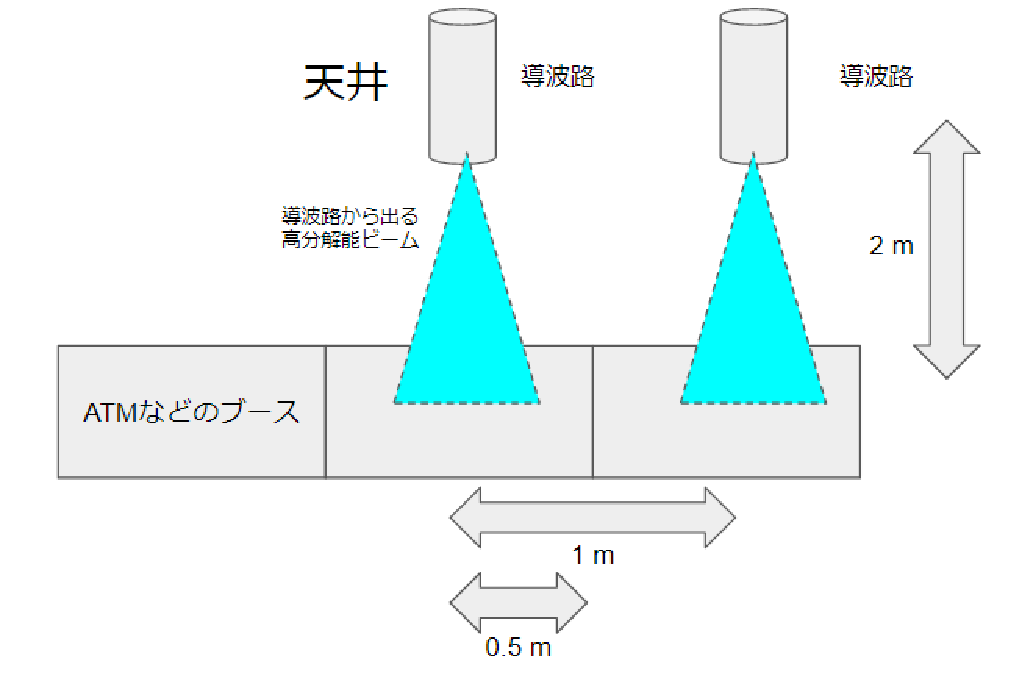
\includegraphics[bb=0 0 384 262, width=0.7\linewidth]{img/usecase.pdf}
    \caption{天井から各ブースへ高分解能ミリ波を提供}
    \label{fig:usecase}
  \end{center}
\end{figure}


最近は大勢の人がいるATMの前にて口座情報を確認する、
シェアオフィスにて個人情報を扱う、
など多数の人々・デバイスが存在する環境にて個人情報をやりとりする機会が多い。
その場合普通のワイヤレス通信を使っている場合、電力解析攻撃によって
電波から情報を抜き取られるリスクもある。
高空間分解能のミリ波を利用することで、
大容量通信を可能にしつつ電波のレイヤーにおいて個人情報を守り、
セキュリティへの貢献が可能となる。

例えば図\ref{fig:usecase}のように天井に誘電体導波路を吊るし、
上から高分解能ビームをユーザー・
デバイスに提供することで物理層におけるセキュアな通信を確立できる。
場所によって変わる分解能の要件にも柔軟に対応可能で、
例えば狭いブースが並んでいる場合はより狭いビームを出す導波路を製作する、
などと調整も可能である。
図の誘電体導波路は短くなっているが、
もっと長い誘電体導波路を遠い位置から引きまわすことで、
柔軟にきめ細やかなエリアが構築される。


\section{シミュレーション}

3Dモデルをシミュレータ上でモデリングし、
電磁波の指向性を測定した。
モデルは図\ref{fig:normal}で見られる普通の棒型、
図\ref{fig:cone}で見られるコーン型、
そして図\ref{fig:dome}で見られるドーム型の3つとした。
すべて円形とし、先端形状を取り除いた場合の長さは50mm、
半径は10mmとなるようにした。
対象周波数は58 GHz から 60 GHzとする。
電力を棒の左側についている完全導体から注入し、
右側から放射される電波の指向性を見る。

\begin{figure}[tb]
  %\capwidth=60mm
  %\ecapwidth=60mm
  \begin{center}
    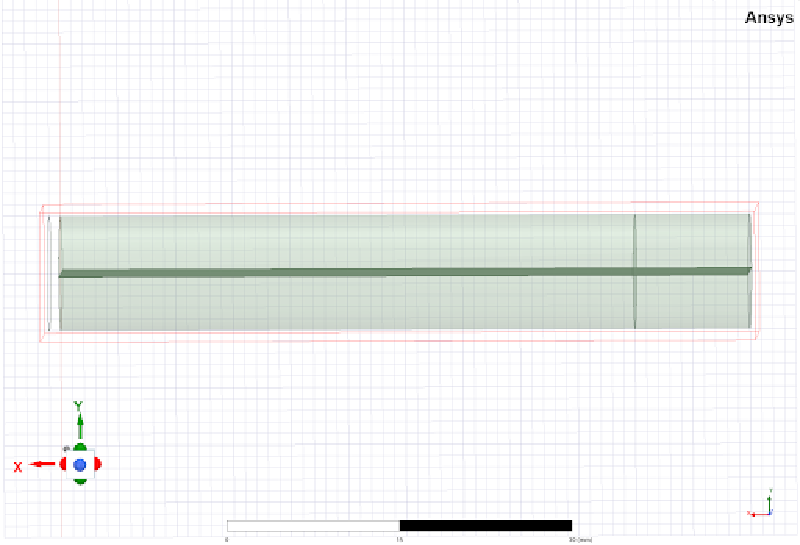
\includegraphics[bb=0 0 384 262, width=0.7\linewidth]{img/normal.pdf}
    \caption{普通の誘電体導波路アンテナ}
    \label{fig:normal}
  \end{center}
\end{figure}

\begin{figure}[tb]
  %\capwidth=60mm
  %\ecapwidth=60mm
  \begin{center}
    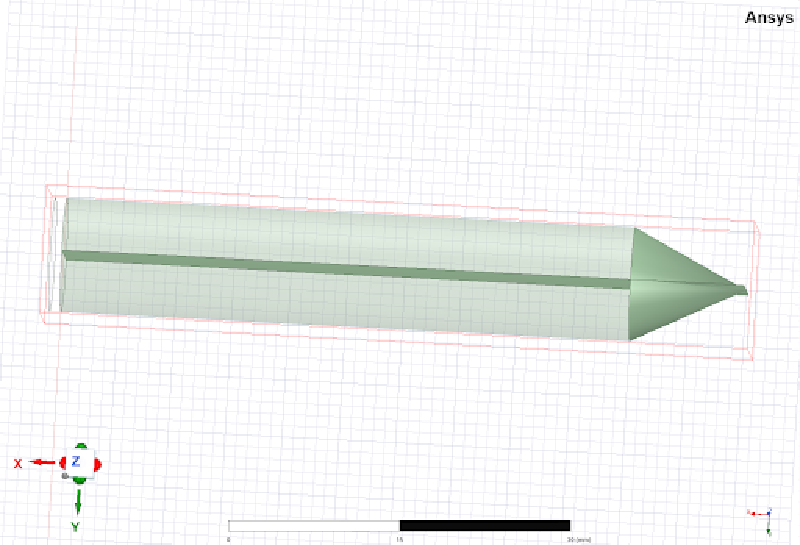
\includegraphics[bb=0 0 384 262, width=0.7\linewidth]{img/cone.pdf}
    \caption{コーン型の誘電体導波路アンテナ}
    \label{fig:cone}
  \end{center}
\end{figure}

\begin{figure}[tb]
  %\capwidth=60mm
  %\ecapwidth=60mm
  \begin{center}
    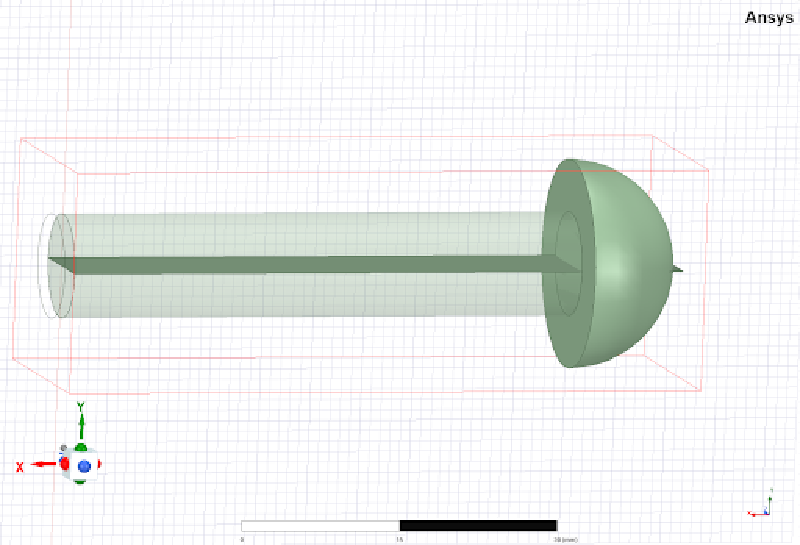
\includegraphics[bb=0 0 384 262, width=0.7\linewidth]{img/dome.pdf}
    \caption{ドーム型の誘電体導波路アンテナ}
    \label{fig:dome}
  \end{center}
\end{figure}

\section{シミュレーションの結果と評価}

50mmで固定した場合については以下の図\ref{fig:directivity_results}のようにドーム型のゲインが一番大きく、
指向性が高くなった。
その次に普通のアンテナ、コーン型のアンテナと続いた。
ドーム型の指向性が一番狭くなった理由としては
レンズアンテナの効果があげられる。
レンズアンテナは開口面アンテナの一種で、
他の開口面アンテナと比較して電波の通路妨害がないので直交偏波を送受でき、
また指向性も高くすることができる。
コーン型については
形状により外側に電波が広がりやすいため、
指向性が広くなったと解釈できる。

\begin{figure}[tb]
  %\capwidth=60mm
  %\ecapwidth=60mm
  \begin{center}
    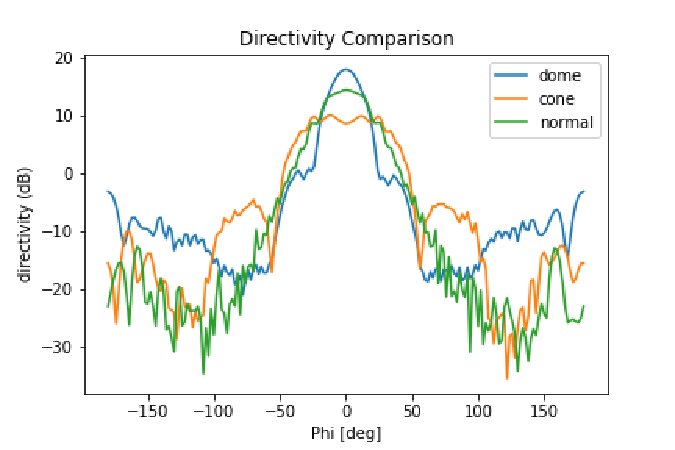
\includegraphics[bb=0 0 324 216, width=1.0\linewidth]{img/directivity.pdf}
    \caption{指向性の結果}
    \label{fig:directivity_results}
  \end{center}
\end{figure}


\section{誘電体導波路アンテナの製作}

シミュレーション結果をもとに誘電体導波路アンテナの製作を行った。
誘電体導波路を加工するとともに、導波管導波路変換器
の製作も必要となった。
誘電体導波路を同軸導波管変換器にそのまま入れた場合、
開口面にて電磁波が散乱してしまい、
電力が逃げてしまう。
電磁波が散乱してしまわないよう、導波路周辺を反射させながら
導波路にまとわりつかせる必要があるため、
導波管から導波路にて変換させる仕組みが必要となる。

また、導波管への挿入する側の導波路の先端を細く削っておく必要がある。
導波管への
導波路の差し込み具合によっても誘電体導波路の反射率は変わるため、
導波路の先端を細くしておくことで
反射率が一番低いところで固定できるようにする。


製作したアンテナについてはSパラメータと指向性を測定した。


電波暗室にて測定した誘電体導波路アンテナの結果は以下となる。

\section{今後の展望}

\subsection{異なる形状での利用の検討}

今回は1次元のPTFEの誘電体導波路の棒に注目して設計と製作を行ったが、
二次元形状であるPTFEのシートを使うことも検討に入れたい。
ドーム型の誘電体導波路アンテナは指向性を高くすることができるものの、
製作の難易度が少しあがってしまう。
二次元のシートの場合はすぐ用意できる上、加工も必要ない。
シートに力を加えたりすることでエリアが構築することが考えられ、
一次元のときに比べてユースケースが広がる。

\subsection{Local5G環境での使用}

今回は電波暗室の遮断された環境で測定を行った。
実際にLocal5Gなどの環境では外部要因が多いため、
分解能と減衰率のパフォーマンスの変動があると予想される。
こちらについての考察も追加できるとよいだろう。

\section{結論}

本研究では電波伝播の直進性や急激な減衰を利活用した誘電体導波路を用いた
ミリ波アンテナを設計し、製作する。
そしてシミュレーション評価だけでなく実際に作製したアンテナを用いた実験により、
有用性を実証する。

本論文の貢献は、まず
鋭いビームを生かして限定したデバイスに情報を渡すことが可能になり、
セキュリティの向上につながることである。
そしてセキュリティの障害となる以下を取り払うことができる。

\begin{itemize}
  \item 誘電体導波路を使うことでハードウェアの開発コストやMIMOの開発コストを抑えることが可能となる
  \item 誘電体導波路はECサイトなどでも購入できるため、リードタイムも縮小できる
  \item 誘電体導波路はある程度曲げても電波の漏れを抑えることができるため、誘電体導波路を室内で引きまわしてミリ波の局所エリアを構築することが可能。
  軽いため、ホーンアンテナなどの既存の機器に比べてエリアをより柔軟に変更できる。
\end{itemize}

\begin{center}
  \Large \textbf{謝辞}
\end{center}

本研究の一部は株式会社NTT Docomoの助成を受けたものです.
共同での実験環境・機材等のご支援を頂き,誠に感謝致します.

%\bibliographystyle{sieicej}
%\bibliography{myrefs}
\bibliography{common_bibliography}

\end{document}
